\documentclass[]{article}

\usepackage[utf8]{inputenc}
\usepackage[T1]{fontenc}

\usepackage{amsmath}
\usepackage{amssymb}
\usepackage{color}
\usepackage{hyperref}
\usepackage{graphicx}
\usepackage{listings}
\usepackage{lstautogobble}
\usepackage{svgcolor}
\usepackage{caption}
\usepackage{subcaption}

\setlength{\parindent}{0cm}

\definecolor{MediumBlue}{rgb}{0.000,0.000,0.804}
\definecolor{DarkGreen}{rgb}{0.000,0.392,0.000}

% Settings for lstlistings
\lstset{%
  basicstyle=\ttfamily,
  columns=fullflexible,
  autogobble,
  keywordstyle=\bfseries\color{MediumBlue},
  stringstyle=\color{DarkGreen},
  commentstyle=\itshape\color{gray},
  tabsize=4
}

%% Listings definition for D programming language
%% Author : Jesse Phillips <Jesse.K.Phillips+D@gmail.com>

\lstdefinelanguage{D}{
  % Keywords
  morekeywords=[1]{
    abstract, alias, align, assert, auto, body, break, cast, catch, class, const,
	 continue, debug, delegate, delete, deprecated, do, else, enum, export,
	 false, final, finally, for, foreach, foreach_reverse, function, goto, if,
	 immutable, import, in, inout, interface, invariant, is, lazy, macro, mixin,
	 module, new, nothrow, null, out, override, package, pragma, private,
	 protected, public, pure, ref, return, shared, static, struct, super,
	 switch, synchronized, template, this, throw, true, try, typedef, typeid,
	 typeof, union, unittest, volatile, while, with
},
  % Special identifiers, common functions
  morekeywords=[2]{enforce},
  % Ugly identifiers
  morekeywords=[3]{
    __DATE__, __EOF__, __FILE__, __LINE__, __TIMESTAMP__, __TIME__, __VENDOR__,
    __VERSION__, __ctfe, __gshared, __monitor, __thread, __vptr, _argptr,
    _arguments, _ctor, _dtor
},
  % Basic types
  morekeywords=[4]{
	 byte, ubyte, short, ushort, int, uint, long, ulong, cent, ucent, void,
	 bool, bit, float, double, real, ushort, int, uint, long, ulong, float,
	 char, wchar, dchar, string, wstring, dstring, ireal, ifloat, idouble,
	 creal, cfloat, cdouble, size_t, ptrdiff_t, sizediff_t, equals_t, hash_t
},
  % Strings
  morestring=[b]{"},
  morestring=[b]{'},
  morestring=[b]{`},
  % Comments
  comment=[l]{//},
  morecomment=[s]{/*}{*/},
  morecomment=[s][\color{blue}]{/**}{*/},
  morecomment=[n]{/+}{+/},
  morecomment=[n][\color{blue}]{/++}{+/},
  % Options
  sensitive=true
}



% Title Page
\title{[WIP] Supplementary material for the transformed density rejection algorithm}
\author{}


\begin{document}
\maketitle

\begin{abstract}
This document aims to provide an understandable guide to the transformed density rejection algorithm and explain all choices made for the mir implementation.
\end{abstract}

\section{Intro to random sampling}

The \href{https://github.com/libmir/mir/pull/240}{code} is currently \textcolor{red}{WIP} and will be available at \texttt{mir.random.flex}. The report \textit{Transformed Density Rejection with Inflection Points} can be found  \href{http://epub.wu.ac.at/3158/1/techreport-110.pdf}{here}.

\subsection{WIP}

If you have ideas how to improve this report, shoot them at me (seb@wilzba.ch).
All code listings can be browsed online at \url{https://github.com/wilzbach/flex-paper}.

\subsection{The problem}

Given a uniform random generator, sample \textit{non-uniform random} values.

The following subsections will introduce some of the basi methods of the
random sampling, which are also used by the Flex algorithm.

\subsection{The inversion method}
\label{subsection:inversion}

The underlying idea of random sampling is that given an inverse function $F^{-1}$ for the cumulative density function (CDF) of a target density $f(x)$, random values can be mapped to a distribution. Given $F^{-1}$ values from the density can be sampled by using the given uniform random generator (of the interval $[0, 1]$).
For example, for the exponential distribution sampling would be:

\begin{lstlisting}[language=D]
S sample(S, RNG, FInv)(RNG gen, FInv finv)
{
    import std.random : uniform;
    S u = uniform!("[]", S)(0, 1);
    return finv(u);
}
import std.random : rndGen;
auto fInvExp = (S x) => -log(S(1) - x);
sample(rndGen, fInvExp)
\end{lstlisting}

More visually you can imagine this with the cumulative plot at \autoref{fig:expo_inv}.
We randomly pick a point $y$ on the CDF graph and then use the \textit{inverse}
function to get the matching value $x$, e.g. if we sample $0.4$ (brown line) the algorithm
would return $-log(1 - 0.4) = 0.51$, for $0.6$ (yellow) it would be $0.91$ and for
$0.9$ (yellow) it would be $2.30$ respectively.

\begin{figure}
    \centering
    \begin{subfigure}[b]{0.49\textwidth}
        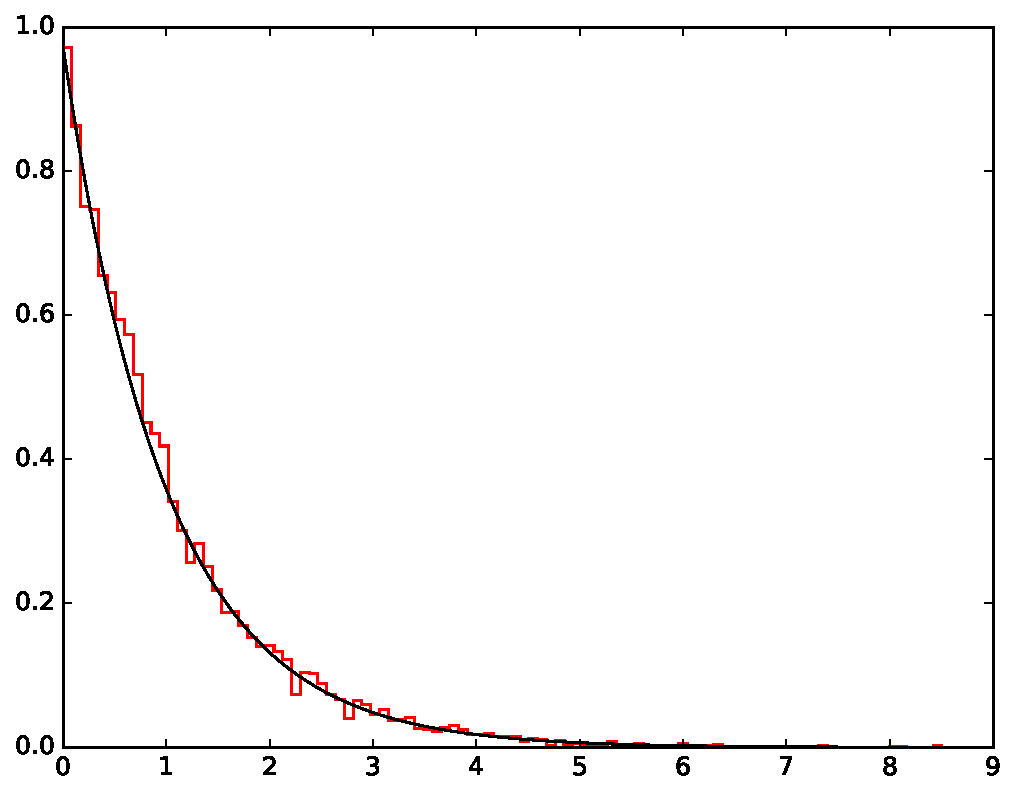
\includegraphics[width=\textwidth]{figs/expo.pdf}
        \caption{Exponential distribution}
    \end{subfigure}
    \begin{subfigure}[b]{0.49\textwidth}
        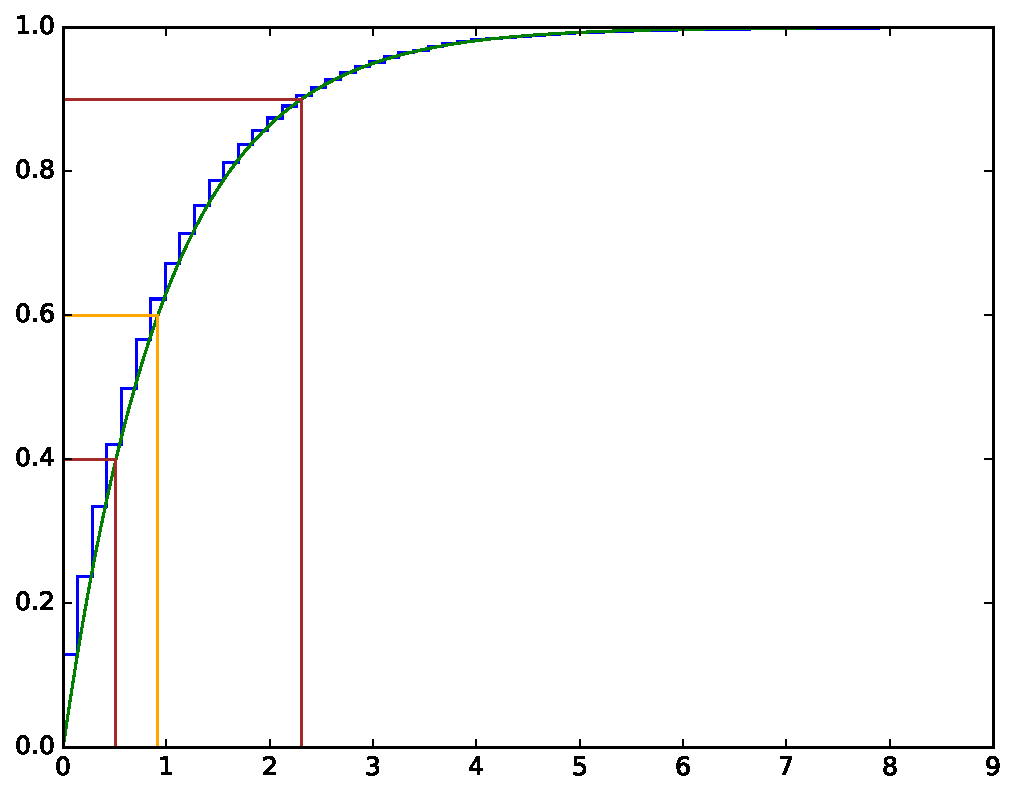
\includegraphics[width=\textwidth]{figs/inversion_sampling.pdf}
        \caption{Exponential distribution, cumlative}
    \end{subfigure}
    \caption{Sampling from the exponential distribution using the inversion method.}
     \label{fig:expo_inv}
\end{figure}

However there are two big problems of the inversion method: (1) for most densities the inverse CDF is not known or can't be determined or (2) if it can be determined it's usually very computationally expensive function (e.g. iterative numeric approximation needs to be used if no exact form can be found).

\subsection{The rejection method}
\label{subsection:rejection}

A very popular alternative is the \textit{rejection} method - often known as \textit{acceptance-rejection} sampling. It only requires one to know the density of a distribution. The general idea is that if a random variable $(x, y)$ is distributed within the density $f$, then it has the density $f$ (blue in \autoref{fig:rejection_method}).

This means we can sample $x$ and $y$ uniformly within the area that is strictly larger than $f$ and check whether the generated point is in the area covered by the density function. If it's within the area the point is \textit{accepted} (black in \autoref{fig:rejection_method}), otherwise it is \textit{rejected} (brown in \autoref{fig:rejection_method})) and new points are sampled until a point, which is within the area and thus can be accepted, is drawn.

More formally, a hat function $h(x)$ that majorizes the density function $f(x)$ is needed. In other words $ \forall x \in [l, r]: f(x) < h(x)$, where $l$ and $r$ are the left and right boundaries of an interval.
The hat function (green in \autoref{fig:rejection_method}) is the boundary function for our target density sampling. In this simple example the hat function would be the horizontal line $x = 1$.

\begin{figure}[h!]
\centering
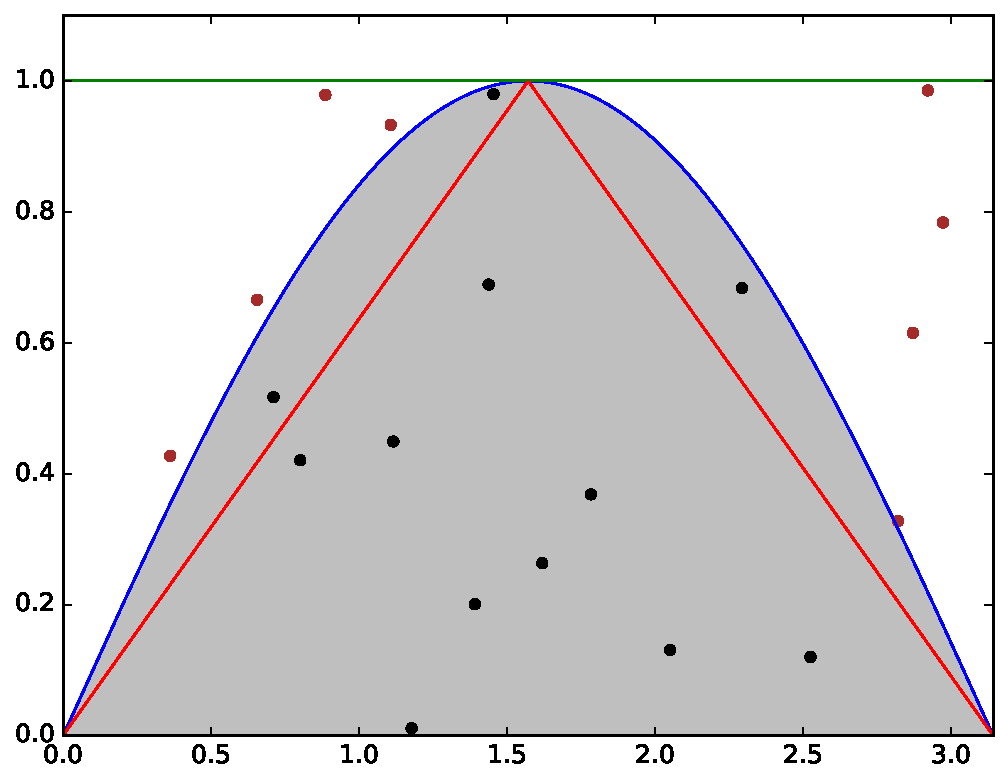
\includegraphics[width=0.8\textwidth]{figs/rejection_sampling.pdf}
\caption{Rejection sampling of $sin(x)$ (blue). Hat function ($x = 1$) is drawn in green, whereas the squeeze function ($1 - |1 - 2x / \pi |$) is drawn in red. Points are marked black when accepted, and brown for rejected.}
\label{fig:rejection_method}
\end{figure}

It is important to see that for every point $x$ we evaluate whether it's within the density area $f(x)$. As $h(x)$ is by definition always larger than $f(x)$ we can use $y * h(x) \leq f(x)$ when we want to programmatically check whether a generated point is within the target density as it covers the entire density of $f(x)$ (as $f(x) \in [0, 1]\  \forall x \in [\ell, r],\  y \in [0, 1]$)

A simplified example of the basic rejection method can be seen here:

\begin{minipage}{\linewidth}
\begin{lstlisting}[language=D]
S sample(RNG, Pdf, Hat, S)(ref RNG gen, Pdf pdf, Hat hat, S left, S right)
{
    import std.random : uniform;
    for (;;)
    {
        // generate x with density proportional to hat(x)
        S x = uniform!("[]", S)(left, right, gen);
        // generate "vertical" variable y to evaluate x
        S y = uniform!("[]", S)(0, 1, gen);
        // check whether the sampled point is within the density
        if (y * hat(x) <= pdf(x))
            return x;
    }
}
alias S = double;
import std.math : PI, sin;
import std.random: rndGen;
auto pdf = (S) => sin(x);
auto hat = (S x) => 1;
sample(rndGen, pdf, hat, S(0), PI);
\end{lstlisting}
\end{minipage}

Furthermore the performance of this method depends heavily on the ratio of $f(x) / h(x) = \alpha$, where $1 / \alpha$ is the average number of needed iterations to sample one value.

\subsection{Rejection with inversion}
\label{subsection:rejection_inversion}

Just a straight line as upper bound yields a lot of uncovered areas, thus a more generic \textit{hat} functions is necessary.
If the inverse of the \textit{hat} function is known, the inversion method can be used to sample from an arbitrary \textit{hat} function:

\begin{minipage}{0.9\linewidth}
\begin{lstlisting}[language=D]
S sample(S, RNG, Pdf, Hat, HatInv)(ref RNG gen, Pdf pdf, Hat hat,
                                       HatInv hatInvCDF)
{
    import std.random : uniform;
    for (;;)
    {
        // generate x with density proportional to hat(x)
        S u = uniform!("[]", S)(0, 1, gen);

		// map u uniquely to a point of the integral of hat(x)
        S x = hatInvCDF(u);

        // generate "vertical" variable y to evaluate x
        S y = uniform!("[]", S)(0, 1, gen);

        // check whether the sampled point is within the density
        if (y * hat(x) <= pdf(x))
            return x;
    }
}
import std.math : PI, sin;
import std.random: rndGen;
alias S = double;
auto pdf = (S) => sin(x);
auto hatInvCDF = (S u) => 0 + u * (PI - 0);
auto hat = (S x) => 1;
sample!S(rndGen, pdf, hat, hatInvCDF);
\end{lstlisting}
\end{minipage}

The (Tin)flex algorithm will show a way to automatically construct a hat function for any differentiable density function.

\subsection{Squeeze functions}
\label{subsection:squeeze}

Calculating the probability density function is often expensive, thus defining a lower bound that can evaluated much faster would be yield a performance boost.
This lower bound is called $s(x)$ which is majorized by $f(x)$, i.e. $s(x) \leq f(x) \forall x \in [l, r]$.
For example, the squeeze function in \autoref{fig:rejection_method} is $1 - |1 - 2x / \pi |$. If $x$ is below the squeeze function, it can be accepted \textit{without} the need to calculate the density function as by definition every point in the squeeze function $s(x)$ is also below $f(x)$. Hence the \textit{sample} routine can be adapted:

\begin{minipage}{0.9\linewidth}
\begin{lstlisting}[language=D]
S sample(S, RNG, Pdf, Hat, HatInv, Squeeze)(ref RNG gen, Pdf pdf,
                              Hat hat, HatInv hatInvCDF, Squeeze sq)
{
    import std.random : uniform;
    for (;;)
    {
        // generate x with density proportional to hat(x)
        S u = uniform!("[]", S)(0, 1, gen);
		// map u uniquely to a point of the integral of hat(x)
        S x = hatInvCDF(u);

        // generate "vertical" variable y to evaluate x
        S y = uniform!("[]", S)(0, 1, gen);
        S t = y * hat(x);

        // check whether the sampled point is below the squeeze
        if (t <= sq(x))
            return x;

        // check whether the sampled point is within the density
        if (y * hat(x) <= pdf(x))
            return x;
    }
}

import std.math : abs, PI, sin;
import std.random: rndGen;
alias S = double;
auto hatInvCDF = (S u) => 0 + u * (PI - 0);
auto hat = (S x) => 1;
auto sq = (S x) => 1 - abs(1 - 2 * x / PI);
sample!S(rndGen, (S) => sin(x), hat, hatInvCDF, sq);
\end{lstlisting}
\end{minipage}


\subsection{Composition}
\label{subsection:composition}

A density function might be split into multiple parts with each having it's own hat and squeeze.
If we are given multiple densities, we can sample from the overall density by picking from each sampler according to a given probability $p_i$ which is defined by their hat area.
For example, \autoref{fig:dist_composition} shows a distribution that is composed out of multiple hat and squeeze parts.

\begin{figure}[h!]
\centering
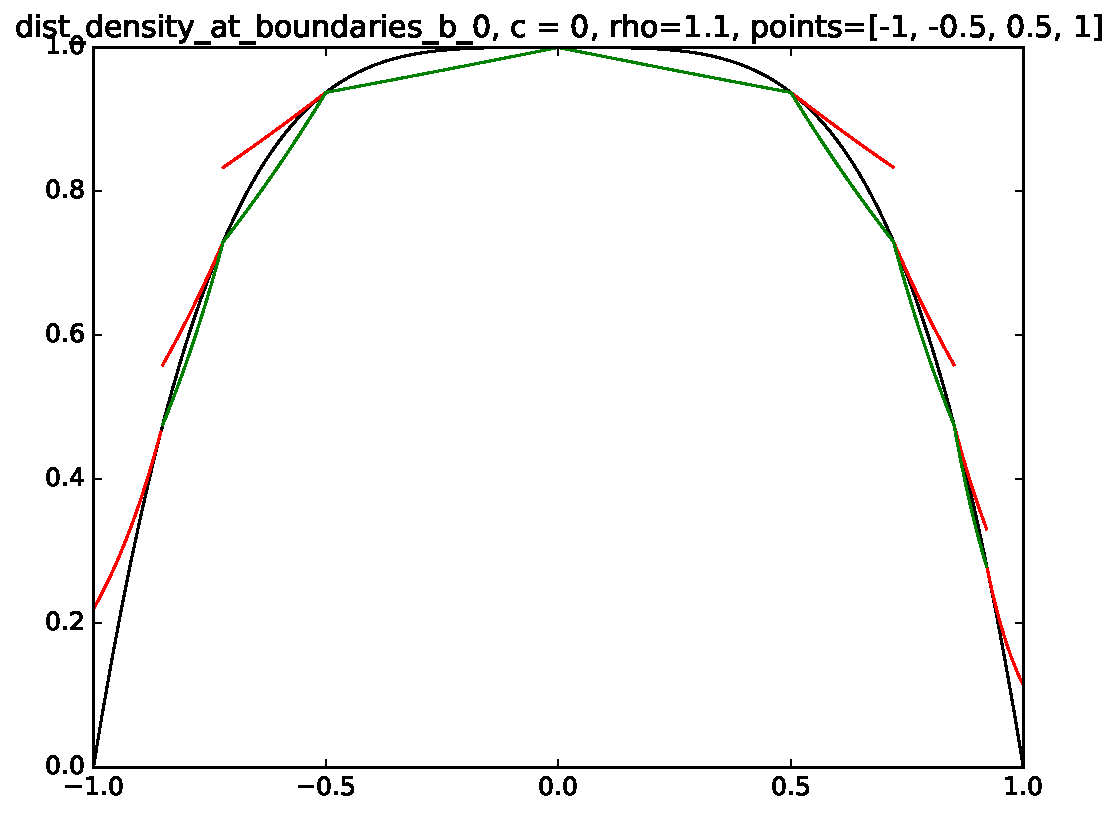
\includegraphics[width=0.8\textwidth]{figs/dist_density_at_boundaries_b_0_hs.pdf}
\caption{Distribution split into multiple hat (red) and squeeze (green) functions.}
\label{fig:dist_composition}
\end{figure}

The idea of composing distributions will be illustrated as follows.
The density function is composed out of an exponential distribution (left) and a uniform distribution (right) and features a gap in the middle.

\pagebreak

%\begin{minipage}{0.9\linewidth}
\begin{lstlisting}[language=D]
S sample(S, RNG, Sampler)(ref RNG gen, Sampler[] samplers, S[] probs)
{
    import mir.random.discrete : discrete;
    // pick a sampler with prob_i
    auto ds = discrete(probs);
    // sample with the chosen sampler
    return samplers[ds(gen)](gen);
}

import std.random: Mt19937, uniform, rndGen;
alias S = double;

alias Sampler = S delegate(ref typeof(gen) gen);
S[] probs = [0.7, 0.3];
Sampler[] samplers = new Sampler[probs.length];

// a part of the exponential distribution on the left
samplers[0] = (ref typeof (gen) gen) {
    import std.math : log;
    auto finv = (S x) => -log(S(1) - x);
    S u = uniform!("[)", S)(0, 0.8);
    return finv(u);
};

// a uniform sampler on the right half
samplers[1] = (ref typeof (gen) gen) {
    return uniform!("[]", S)(2, 3, gen);
};
sample!S(gen, samplers, probs);
\end{lstlisting}
%\end{minipage}

\ \\

The result of our basic composition with different target probabilities for the samples can be seen in \autoref{fig:composition_exp_uniform}. The (Tin)flex algorithm will automatically generate intervals with hat and squeeze function for the desired distribution that are connected with such a composition sampler.

\begin{figure}[h]
    \centering
    \begin{subfigure}[b]{0.49\textwidth}
        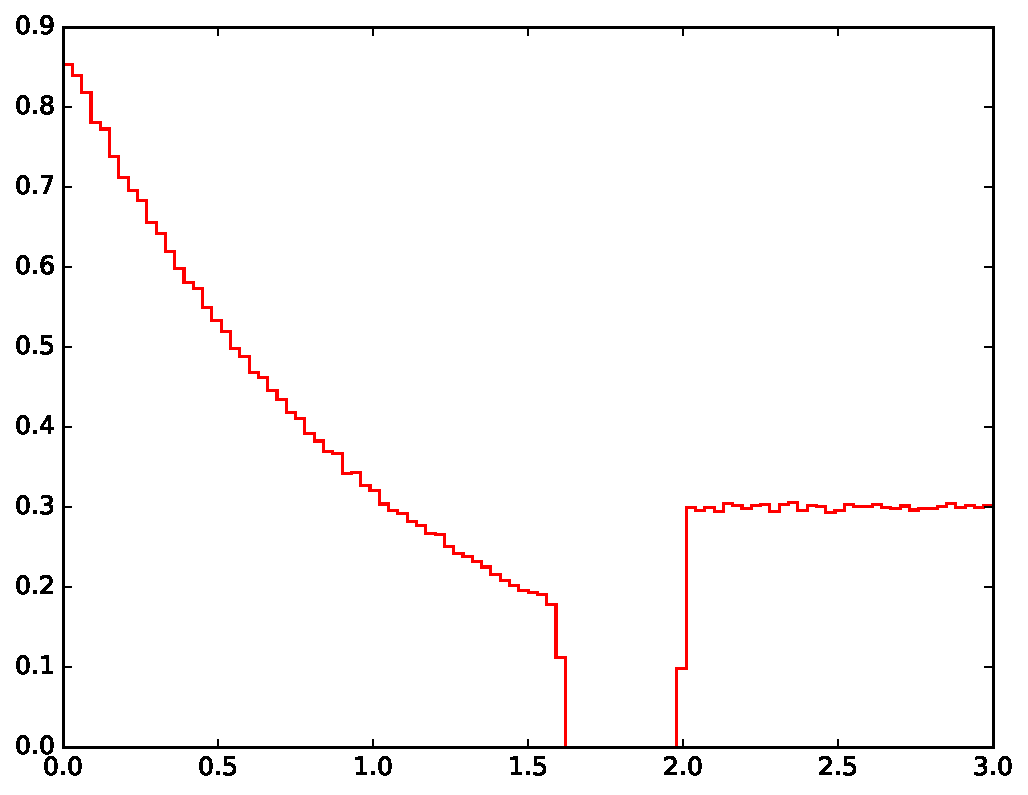
\includegraphics[width=\textwidth]{figs/composed_dist_70_30.pdf}
        \caption{$p = [0.7, 0.3]$}
    \end{subfigure}
    \begin{subfigure}[b]{0.49\textwidth}
        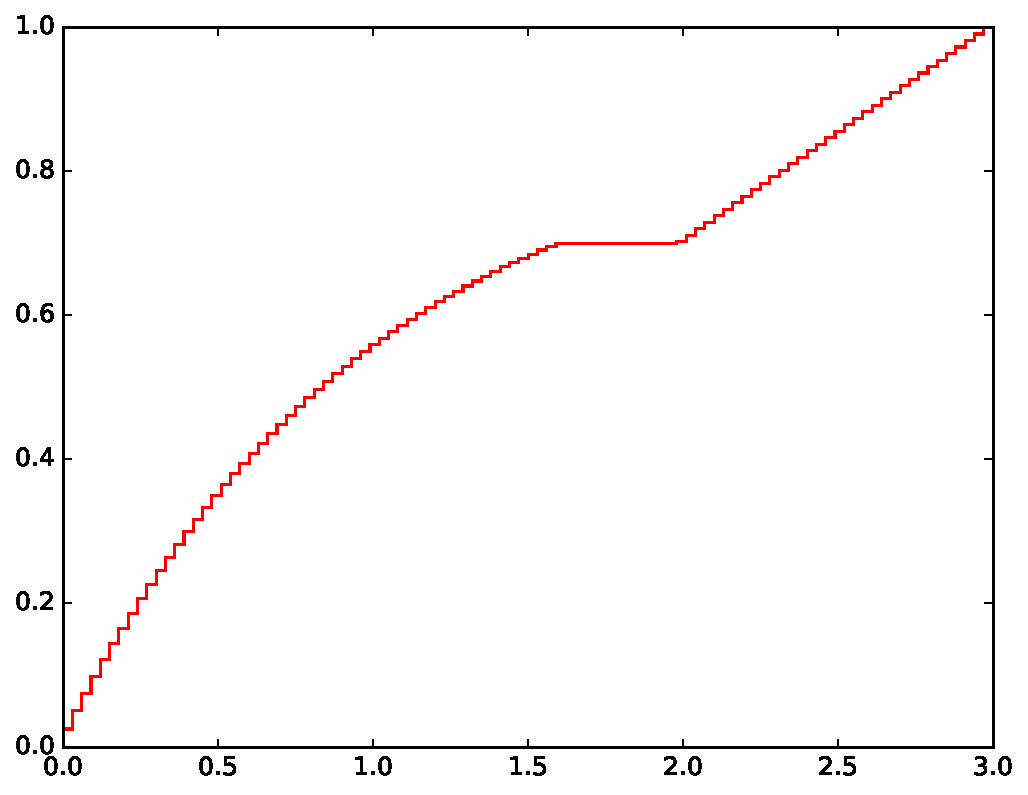
\includegraphics[width=\textwidth]{figs/composed_dist_70_30_cum.pdf}
        \caption{$p = [0.7, 0.3]$, cumlative}
    \end{subfigure}
    \centering
    \begin{subfigure}[b]{0.49\textwidth}
        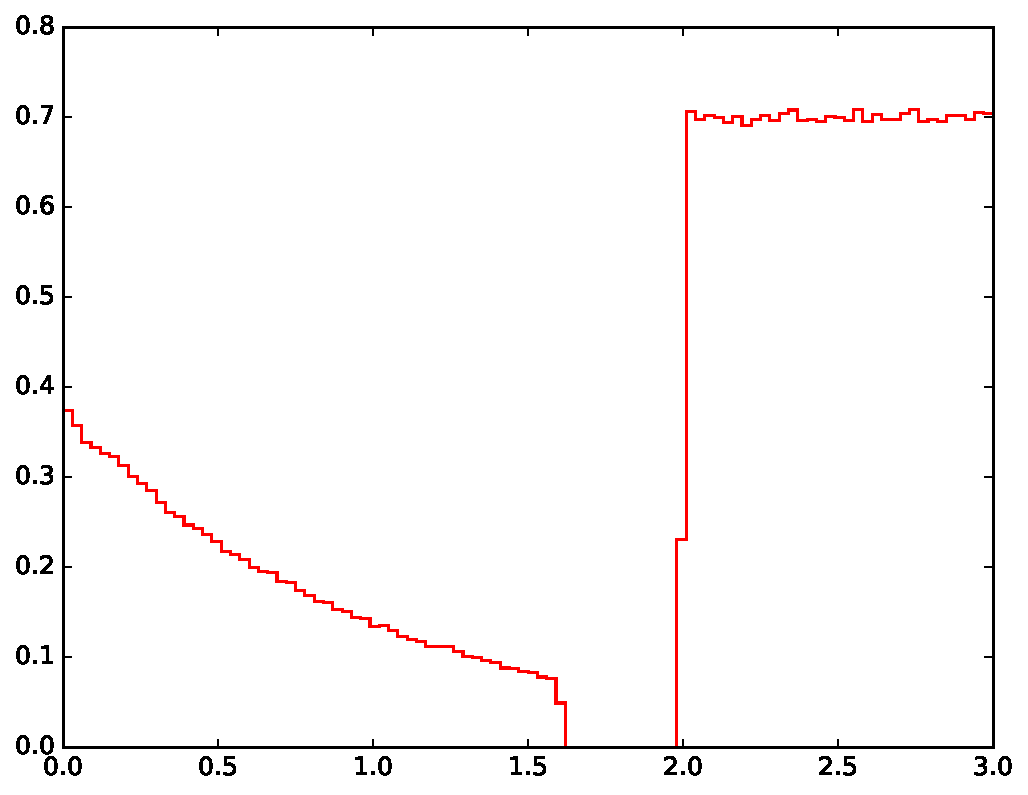
\includegraphics[width=\textwidth]{figs/composed_dist_30_70.pdf}
        \caption{$p = [0.3, 0.7]$}
    \end{subfigure}
    \begin{subfigure}[b]{0.49\textwidth}
        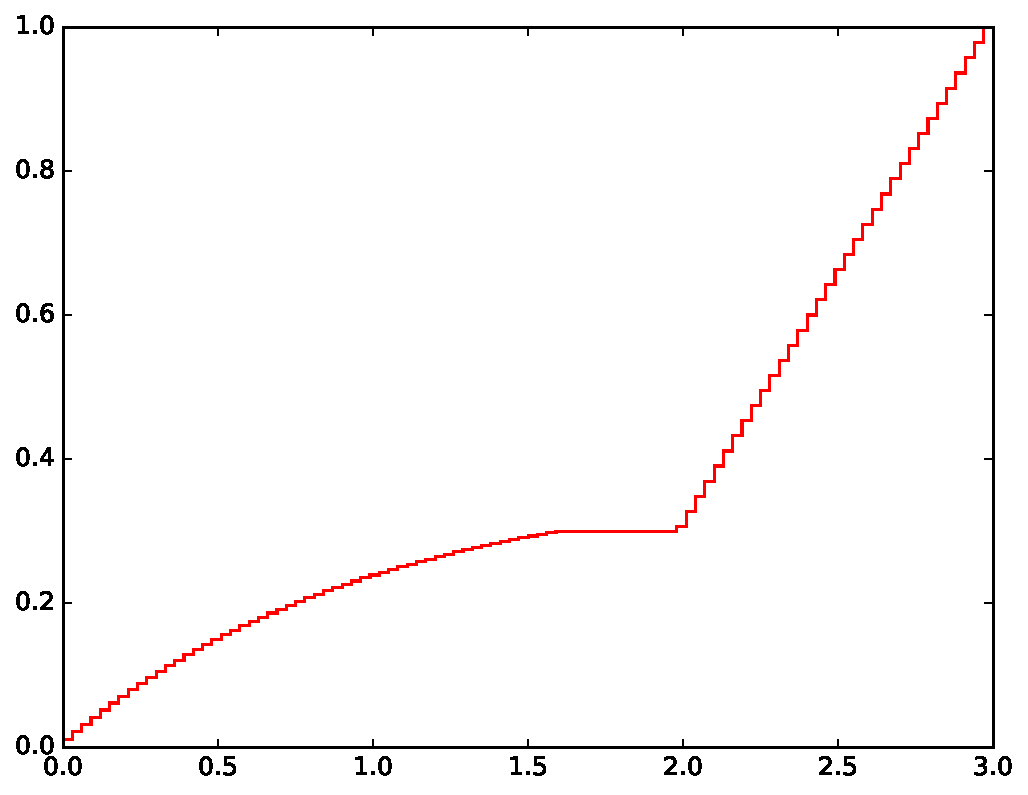
\includegraphics[width=\textwidth]{figs/composed_dist_30_70_cum.pdf}
        \caption{$p = [0.3, 0.7]$, cumulative}
    \end{subfigure}
    \caption{Composition of exponential and uniform distribution}
     \label{fig:composition_exp_uniform}
\end{figure}



\section{Intro to (Tin)flex}

\subsection{Idea}

Split the density distribution into multiple intervals for which better approximation for the \textit{hat} and \textit{squeeze} function can be constructed. Sample from the intervals using \textit{composition} and then for the selected intervals sample a value $x$ using the \textit{rejection with inversion} method.
For example in \autoref{fig:tf_example_normal} the normal distribution is split into six intervals with different hat and squeeze functions. The efficiency of the sampling can iteratily be improved by splitting more intervals and thus yielding a better approximation to the density.

\begin{figure}
    \centering
    \begin{subfigure}[b]{0.49\textwidth}
        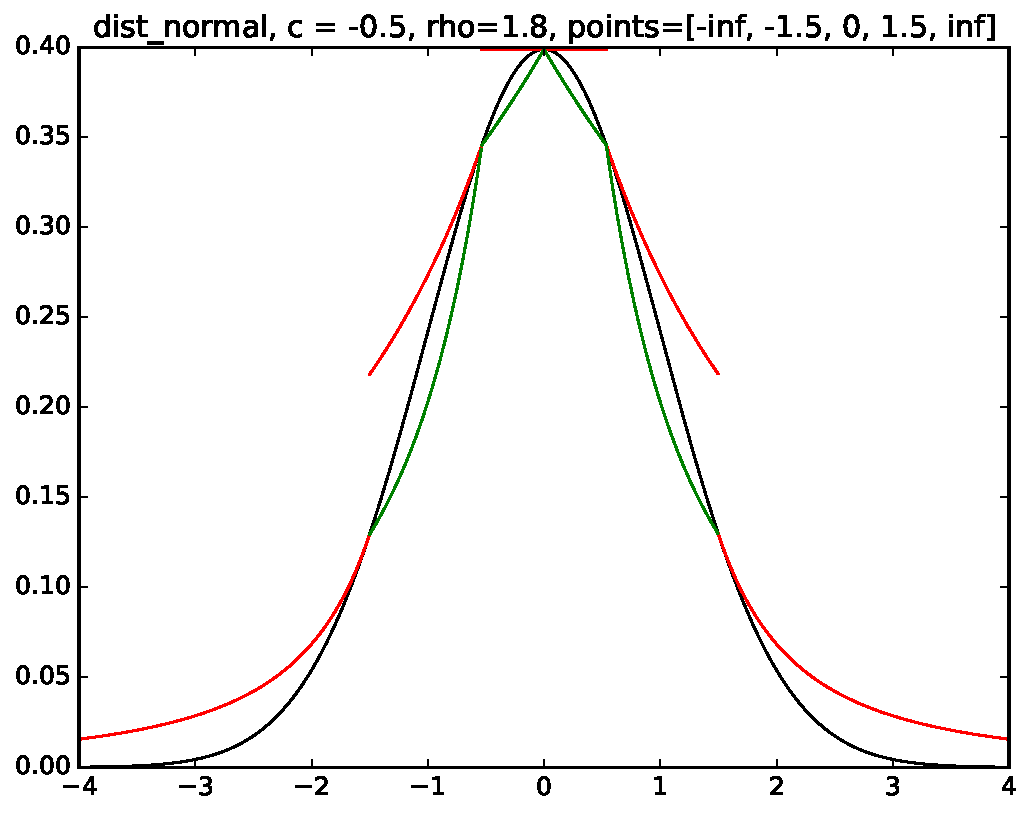
\includegraphics[width=\textwidth]{figs/tf_example_normal_6.pdf}
        \caption{$\rho = 1.8$, 6 intervals constructed}
    \end{subfigure}
    \begin{subfigure}[b]{0.49\textwidth}
        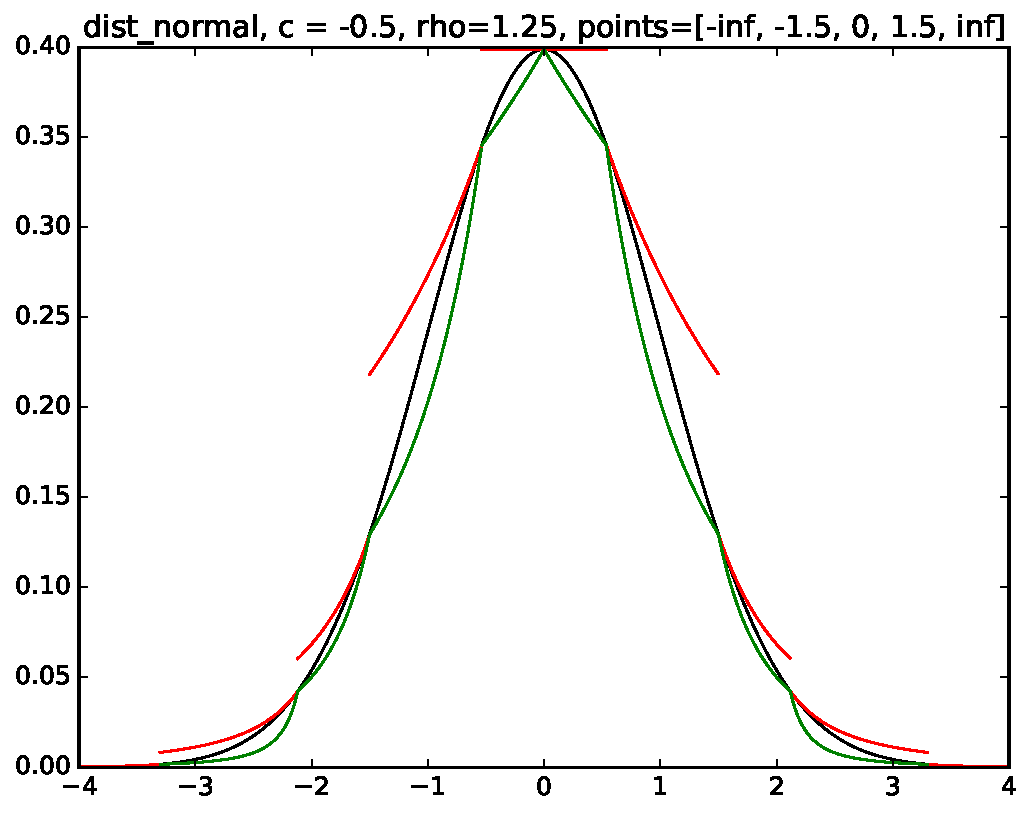
\includegraphics[width=\textwidth]{figs/tf_example_normal_10.pdf}
        \caption{$\rho = 1.25$, 10 intervals constructed}
    \end{subfigure}
    \centering
    \begin{subfigure}[b]{0.49\textwidth}
        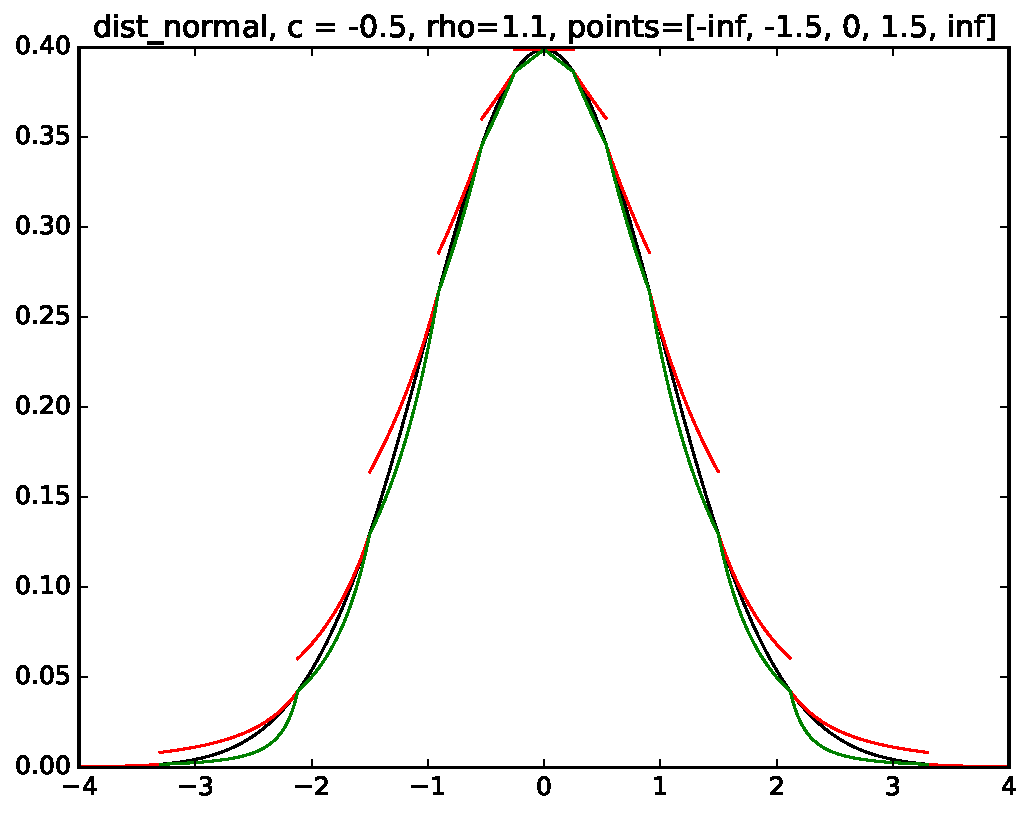
\includegraphics[width=\textwidth]{figs/tf_example_normal_14.pdf}
        \caption{$\rho = 1.1$, 14 intervals constructed}
    \end{subfigure}
    \begin{subfigure}[b]{0.49\textwidth}
        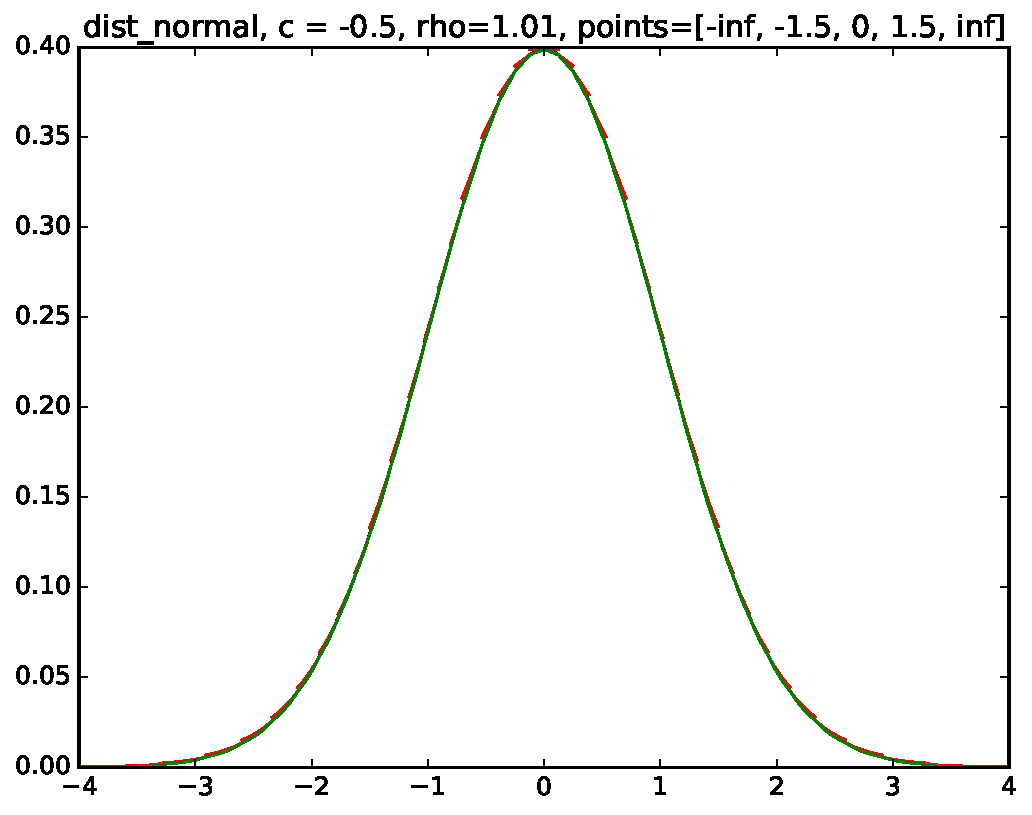
\includegraphics[width=\textwidth]{figs/tf_example_normal_44.pdf}
        \caption{$\rho = 1.01$, 44 intervals constructed}
    \end{subfigure}
    \caption{Flex algorithm for the normal distribution with different efficiencies $\rho$}
     \label{fig:tf_example_normal}
\end{figure}

\subsection{Transformations}

To approximate the hat and squeeze function Tinflex constructs linear functions when an interval is either concave or convex.
However as most distributions aren't \textit{concave}, but \textit{log-concave}, Tinflex uses a family of transformation of the pdf function as it operates in \textit{logspace} and can thus "force" most distributions to be concave. The transformations can be grouped in two classes:

\subsubsection{$c \neq 0$}

The general transformation function is $x^c$, however as inverse function is only defined in $\mathbb{C}$, we need to restrict it to positive numbers.

\[T_c(x) = sgn(c) * x^c\]

With the usual inversion rules we get if $c > 0$

\begin{align*}
y &= x^c \\
log(y) &= log(x^c) \\
log(y) &= c * log(x) \\
\frac{log(y)}{c} &= log(x) \\
exp\left(\frac{log(y)}{c}\right) &= x
\end{align*}

which is $y^{1 / c}$ and if $c < 0$:

\begin{align*}
y &= -x^c \\
log(y) &= log(-x^c) \\
log(y) &= -c * log(x) \\
\frac{log(y)}{c} &= -log(x) \\
exp\left(\frac{log(y)}{c}\right) &= -x
\end{align*}

which is $(-y)^{1 / c}$.
Thus in general we can define the inverse function as:

\[T_c^{-1}(x) = (sgn(c) * x)^{\frac{1}{c}}\]

An example of $T_c$ with $c = 2$ can be seen in \autoref{fig:sgn_pow} and for $c = -0.5$ in \autoref{fig:sgn_pow_0_5}.

Please note that (1) in the Tinflex paper and below this case is split into multiple common cases to have simpler formulas and reduce numerical errors. Furthermore (2) only with $c = 0$ the transformation is two-sided, thus for $c < 0$ $T^{-1}(x)$ is only defined for $x < 0$ in $\mathbb{R}$.

\begin{figure}[h!]
\centering
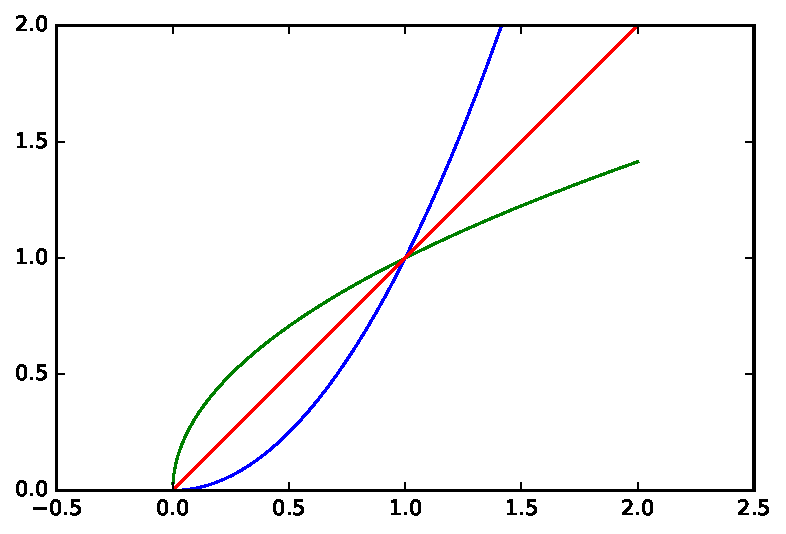
\includegraphics[width=0.8\textwidth]{figs/a_2_sgn_pow.pdf}
\caption{$x^2$ (red) and it's inverse $x^{1/2}$ (blue)}
\label{fig:sgn_pow}
\end{figure}

\begin{figure}[h!]
\centering
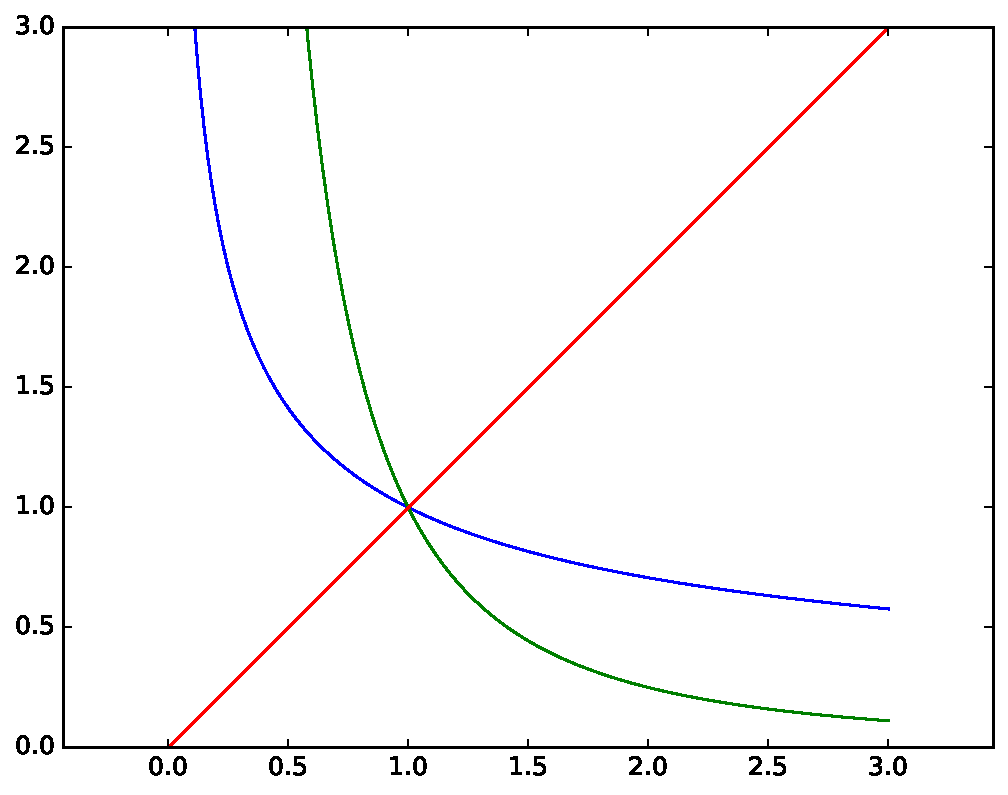
\includegraphics[width=0.8\textwidth]{figs/a_0_5_sgn_pow.pdf}
\caption{$-x^{-0.5}$ (red) and it's inverse $-x^{1/-0.5}$ (blue)}
\label{fig:sgn_pow_0_5}
\end{figure}

\pagebreak

\ \\

\pagebreak

\subsubsection{$c = 0$}

The special case for $c = 0$ needs to be made as division by zero isn't defined, however with this case the natural logarithm and exponential function is used.

\[T_c(x) = log(x)  \]

and it's inverse:

\[T_c^{-1}(x) = exp(x) \]

\begin{figure}[h]
\centering
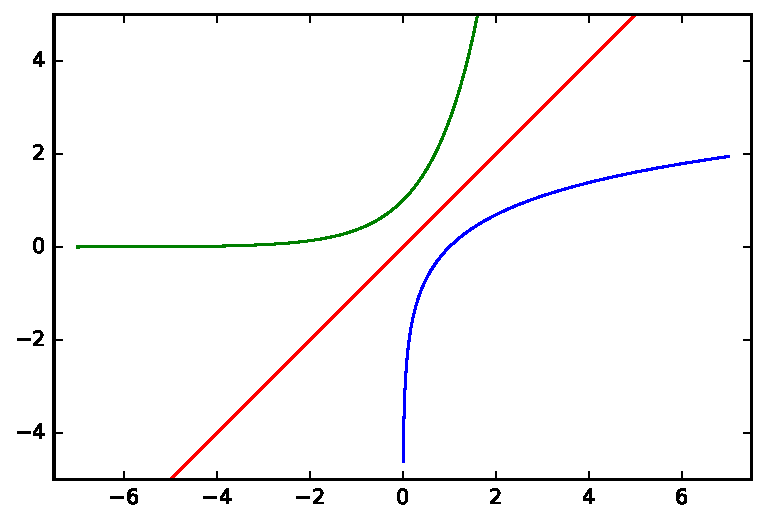
\includegraphics[width=0.8\textwidth]{figs/log_exp}
\caption{Exponential function (red) and it's inverse the natural log (blue)}
\label{fig:log_exp}
\end{figure}

\ \\

Moreover in accordance to the Tinflex paper $f(x)$ is the pdf, and $\tilde{f}(x)$ is its transformation.

\[\tilde{f}(x) = T_c(f(x))  \]

\subsubsection{Input of Tinflex}

Tinflex expects the \textbf{log}-density, which means that for $c = 0$, no transformations need to be applied.
However for $c \neq 0$ the inverse is needed, we first need to apply the \textit{inverse} $T_c^{-1}(x) = exp(x)$ and then apply the other $T_c$ transformation:

\begin{align*}
\tilde{f}(x) &= T_{c \neq 0}(T_0^{-1}(x))) \\
&= T_{c \neq 0}(exp(x))) \\
&= sgn(c) * exp(x)^c \\
&= sgn(c) * exp(x *c)
\end{align*}

\subsection{Linear functions}

The Tinflex paper uses the following definition for linear functions which are used in parts to construct hat and squeeze functions. The hat function majorizes the \textit{transformed} pdf, whereas the \textit{transformed} pdf majorizes the squeeze function.

\[ \tilde{f}(x) = \alpha + \beta * (x - x_0) \]

In the latter $h(x)$ will also be used instead of $\tilde{f}(x)$.
Remember that the transformation is applied with $T_c(x)$.

\subsection{Construction of linear functions}

For both secants and tangents $x_0$ and $\alpha$ within the interval $[\ell, r]$ are defined as follows:

\begin{enumerate}
\item $x_0$ is $\ell$ if $\tilde{f}(\ell) >= \tilde{f}(r)$, $r$ otherwise
\item $\alpha = \tilde{f}(x_0)$
\end{enumerate}

In fact only $\beta$ is defined differently: \\ 
\ \\
Tangent: $\beta = \tilde{f}'(x_0)$ \\ 
Secant:  $\beta = \frac{\tilde{f}(r) - \tilde{f}(\ell)}{r - \ell}$




\section{Area $A_h$}

For the sampling we want to be able to compute the inverse CDF for any $x$ in a choosen interval.

The area below a constructed hat function (and thus respectively for the squeeze function) within the interval $[\ell, r]$ can be calculated by its definite integral. $F_{T_c}$ is the antiderivative (aka primitive integral) of the inverse transformation $T^{-1}$ as $h(x) = T^{-1}(\tilde{h}(x))$ and $F_{T_c}(x) = \int_{-\infty}^{x} T^{-1}(t) dt$. Note that $\tilde{h}(x)' = \beta$.

\begin{align*}
A_h &= \int_{\ell}^{r} h(x) dx \\
	&= \int_{\ell}^{r} T^{-1}(\tilde{h}(x)) * \frac{\tilde{h'}(x)}{\tilde{h}'(x)} dx \\
	&= \int_{\ell}^{r} (F_T(\tilde{h}(x))' * \frac{1}{\tilde{h}'(x)} dx \\
&= \frac{1}{\beta} \big( F_{T_c} (\tilde{h}(r)) - F_{T_c}(\tilde{h}(\ell)) \big)
\end{align*}

The CDF $H_i(x)$ with $x \in [l_i, r_i]$ is thus:

\[ \frac{1}{\beta} \big( F_{T_c} (\tilde{h}(x)) - F_{T_c}(\tilde{h}(\ell)) \big) \]

with $H_i(r_i) = A_h$.


Note that $H_(x)$ is only defined if $\beta \neq 0$.

\subsection{c = 1}

From  $T^{-1} = x$ follows trivially its integral $F_{T_1} = \frac{1}{2} * x^{\frac{2}{1}}$
and then we can simplify the above equation to:

\begin{align*}
A_h &= \frac{1}{\beta} \big(F_{T_1}(h(r)) - F_{T_1}(h(\ell)) \big) \\
&= \frac{1}{\beta} \left(0.5 * (\alpha + \beta * (r - x_0))^2 - 0.5 * (\alpha + \beta * (\ell - x_0))^2 \right) \\
\end{align*}

\subsubsection{Z-Trick}

Z-Trick, $x_0$ can only be either $r$ or $\ell$, thus either $r - x_0$ or $\ell - x_0$ is zero. \\

\textbf{$I) \quad x_0 = \ell$}

\begin{align*}
A_h &= \frac{0.5}{\beta} \left( (\alpha + \beta * (r - \ell))^2 - \alpha^2  \right) \\
&= \frac{0.5}{\beta} \left( \alpha^2 + 2 * \alpha * \beta * (r - \ell) + (\beta * (r - \ell))^2 - \alpha^2  \right) \\
&= \frac{0.5}{\beta} \left( 2 * \alpha * \beta * (r - \ell) + (\beta * (r - \ell))^2 \right) \\
&= 0.5 * \left( 2 * \alpha * (r - \ell) + \beta * (r - \ell)^2 \right) \\
&= 0.5 * (r - \ell) * \left( 2 * \alpha  + \beta * (r - \ell) \right) \\
&= (r - \ell) * \left(\alpha  + 0.5 * \beta * (r - \ell) \right) \\
\end{align*}

\textbf{$II) \quad x_0 = r$}

\begin{align*}
A_h &= \frac{0.5}{\beta} \left( \alpha^2 - (\alpha + \beta * (\ell - r))^2 \right) \\
&= \frac{0.5}{\beta} \left( \alpha^2 - \alpha^2 - 2 * \alpha * \beta * (\ell - r) - (\beta * (\ell - r))^2   \right) \\
&= \frac{0.5}{\beta} \left( - 2 * \alpha * \beta * (\ell - r) - (\beta * (\ell - r))^2 \right) \\
&= -0.5 * \left( 2 * \alpha * (\ell - r) + \beta * (\ell - r)^2 \right) \\
&= -0.5 * (\ell - r) * \left( 2 * \alpha  + \beta * (\ell - r) \right) \\
&= - (\ell - r) * \left( \alpha  + 0.5 * \beta * (\ell - r) \right) \\
&= (r - \ell) * \left( \alpha  + 0.5 * \beta * (\ell - r) \right) \\
\end{align*}

this means with a helper function $\sigma(x)$ which is

\[
	\sigma(x) =
	\begin{cases}
		1 & \text{for } x = \ell \\
		-1 & \text{for } x = r \\
	\end{cases}
\]

we can summarize this in one equation:

\[
	A_{h_1} = (r - \ell) * \left( \alpha  + 0.5 * \beta * \sigma(x) * (r - \ell) \right) \\
\]

\subsection{c = 0}

$F_{T_0} = e^x$

\begin{align*}
A_{h_0} &= \frac{1}{\beta} \left( e^{h(r)} - e^{h(\ell)} \right)
\end{align*}

First we simplify the equation a bit:

\begin{align*}
A_{h_0} &= \frac{1}{\beta} \left( e^{h(r)} - e^{h(\ell)} \right) \\
	&= \frac{1}{\beta} \left( e^{\alpha + \beta (r - x_0)} - e^{\alpha + \beta (l - x_0)} \right) \\
	&= \frac{1}{\beta} \left( e^{\alpha + \beta r - \beta x_0} - e^{\alpha + \beta l - \beta x_0} \right) \\
	&= \frac{1}{\beta} \left( e^{\alpha} * e^{\beta r} * e^{-\beta x_0} - e^{\alpha} * e^{\beta l} * e^{- \beta * x_0} \right) \\
	&= \frac{1}{\beta} \left( e^{\alpha - \beta x_0} * \left(e^{\beta r} - e^{\beta \ell} \right) \right) \\
\end{align*}

Again we use the z-trick to distinguish between both cases.


I) $x_0 = \ell$:

\begin{align*}
	A_{h_0} &= \frac{1}{\beta} \left( e^{\alpha - \beta * x_0} * \left(e^{\beta r} - e^{\beta \ell} \right) \right) \\
	&= \frac{1}{\beta} \left( e^{\alpha - \beta * \ell} * \left(e^{\beta r} - e^{\beta \ell} \right) \right) \\
	&= \frac{1}{\beta} \left(e^{\alpha - \beta \ell - \beta r} - e^{\alpha - \beta \ell + \beta \ell} \right) \\
	&= \frac{1}{\beta} \left(e^{\alpha - \beta \ell - \beta r} - e^{\alpha} \right) \\
	&= \frac{e^{\alpha}}{\beta} \left(e^{- \beta \ell - \beta r} - 1) \right) \\
	&= \frac{e^{\alpha}}{\beta} \left(e^{\beta (r - \ell)} - 1 \right) \\
\end{align*}

With Taylor-Series of $n = 4$ with $k = \beta (r - \ell)$ and $e^{\alpha} = g(x)$ we can approximate this arbitrarily,
e.g. for $n = 3$,

\begin{align*}
	A_{h_0} &= \frac{e^{\alpha}}{\beta} \left(1 + k + \frac{k^2}{2} +  \frac{k^3}{6} - 1 \right)
\end{align*}

and for more precision we can increase $n$ to $4$.

\begin{align*}
	A_{h_0} &= \frac{e^{\alpha}}{\beta} \left(1 + k + \frac{k^2}{2} +  \frac{k^3}{6} + \frac{k^4}{24} - 1 \right)
\end{align*}

%\textcolor{red}{TODO: Show that this does make a difference}

II) $x_0 = r$:

\begin{align*}
	A_{h_0} &= \frac{1}{\beta} \left( e^{\alpha - \beta * x_0} * \left(e^{\beta r} - e^{\beta \ell} \right) \right) \\
	&= \frac{1}{\beta} \left( e^{\alpha - \beta * r} * \left(e^{\beta r} - e^{\beta \ell} \right) \right) \\
	&= \frac{1}{\beta} \left(e^{\alpha - \beta r - \beta r} - e^{\alpha - \beta r + \beta \ell} \right) \\
	&= \frac{1}{\beta} \left(e^{\alpha} - e^{\alpha - \beta r + \beta \ell} \right) \\
	&= \frac{e^{\alpha}}{\beta} \left(1 - e^{- \beta r + \beta \ell} ) \right) \\
	&= \frac{e^{\alpha}}{\beta} \left(1 - e^{\beta (\ell - r)}  \right) \\
\end{align*}

hence in general

\[
	\frac{e^{\alpha} * \sigma(x)}{\beta} \left(e^{\beta * \sigma(x) (r - \ell)} - 1 \right) \\
\]

and thus:

\[
	A_{h_0} = \frac{e^{\alpha}}{\beta} * \sigma(x) * \left(e^{\beta * \sigma(x) (\ell - r)} - 1 \right)
\]

and with Taylor-series:

\begin{align*}
	A_{h_0} &= \frac{e^{\alpha} * \sigma(x)}{\beta} \left(1 + k + \frac{k^2}{2} +  \frac{k^3}{6} + \frac{k^4}{24} - 1 \right)
\end{align*}

where $k = \beta * \sigma(x) * (r - l)$

\subsection{c = -0.5}

$T_{-0.5}^{-1} = \frac{1}{x^2}$, hence $F_{T_{-0.5}} = - \frac{1}{x}$


\subsubsection{Z-trick}


\begin{align*}
A_h &= \frac{1}{\beta} \left(\frac{-1}{\tilde{h}(r)} - \frac{-1}{\tilde{h}(\ell)} \right) \\
& = \frac{1}{\beta} \left(- \frac{1}{\tilde{h}(r)} + \frac{1}{\tilde{h}(\ell)} \right) \\
& = \frac{1}{\beta} \left(\frac{1}{\tilde{h}(l)} - \frac{1}{\tilde{h}(r)} \right)
\end{align*}

\subsubsection{Z-trick}

I) $x_0 = \ell$

\begin{align*}
	A_{h_{-0.5}} & = \frac{0}{\beta} \left(\frac{1}{\alpha} - \frac{1}{\alpha - (\beta * (\ell - r)} \right) \\
	& = \frac{1}{\alpha \beta} - \frac{1}{\alpha \beta - (\beta^2 * (\ell - r)} \\
	& = \frac{\alpha \beta - (\beta^2 * (\ell - r)}{(\alpha \beta) * (\alpha \beta - (\beta^2 * (\ell - r))} - \frac{\alpha \beta}{\alpha \beta * ( \alpha \beta - (\beta^2 * (\ell - r))} \\
	& = \frac{-\beta^2 * (\ell - r)}{\alpha \beta * \alpha \beta - \alpha \beta (\beta^2 * (\ell - r))}\\
	& = \frac{-(\ell - r)}{\alpha^2 - \alpha \beta (\ell - r)}\\
	& = \frac{r - \ell}{\alpha^2 + \alpha \beta (r - \ell)}\\
\end{align*}

II) $x_0 = r$

\begin{align*}
A_{h_{-0.5}} & = \frac{1}{\beta} \left(\frac{1}{\alpha - (\beta * (r - \ell)} - \frac{1}{\alpha} \right) \\
\end{align*}

and thus in general:

\begin{align*}
	A_{h_{-0.5}} & = \frac{r - \ell}{\alpha^2 + \alpha \beta * \sigma(x) * (r - \ell)}\\
\end{align*}







\subsection{c = -1}

$T_{-1} = -\frac{1}{x}$, thus its integral $F_{T_{-1}} = - log(-x)$

\begin{align*}
	A_{h_{-1}} &= \frac{1}{\beta} \left(-log(-\tilde{h}(r)) + log(-\tilde{h}(l)) \right) \\
&= \frac{1}{\beta} \left(-log(-\alpha - (\beta * (r - \ell))) + log(-\alpha) \right)
\end{align*}

we use the Z-trick again:

I) $x_0 = \ell$

\begin{align*}
	A_{h_{-1}} &= \frac{1}{\beta} \left(-log(-\tilde{h}(r)) + log(-\tilde{h}(l)) \right) \\
&= \frac{1}{\beta} \left(-log(-\alpha - (\beta * (r - \ell))) + log(-\alpha) \right)
\end{align*}

II) $x_0 = r$

\begin{align*}
A_{h_{-1}} &= \frac{1}{\beta} \left(- log(-\alpha) + log(-\alpha - (\beta * (\ell - r))) \right)
\end{align*}


and in general:

\[
	A_{h_{-1}} = \frac{\sigma(x)}{\beta} \left(-log(-\alpha - (\beta * \sigma(x) * (r - \ell))) + log(-\alpha) \right)
\]

Please note that if $\beta \sim 0$, this gets undefined. Thus this special case needs to be covered separately.

\subsection{$c > 0$}

$T_c^{-1} = x^{1/c}$, thus it's integral is $F_T = \frac{c}{c + 1} * x^{\frac{c + 1}{c}}$

\begin{align*}
A_h &= \frac{1}{\beta} \left( \frac{c}{c + 1} h(r)^{\frac{c + 1}{c}} - \frac{c}{c + 1} h(\ell)^{\frac{c + 1}{c}} \right) \\
A_h &= \frac{c}{\beta * (c + 1)}  \left( h(r)^{\frac{c + 1}{c}} - h(\ell)^{\frac{c + 1}{c}} \right) \\
\end{align*}

we use the z-trick again:

I) $x_0 = \ell$

\begin{align*}
A_h &= \frac{c}{\beta * (c + 1)}  \left( (\alpha + \beta * (r - \ell))^{\frac{c + 1}{c}} - \alpha^{\frac{c + 1}{c}} \right) \\
\end{align*}

II) $x_0 = r$

\begin{align*}
A_h &= \frac{c}{\beta * (c + 1)}  \left( \alpha^{\frac{c + 1}{c}} - (\alpha + \beta * (\ell - r))^{\frac{c + 1}{c}} \right) \\
\end{align*}

thus in general:

\[
	A_h &= \frac{c * \sigma(x)}{\beta * (c + 1) }  \left( (\alpha + \beta * \sigma(x) * (r - \ell))^{\frac{c + 1}{c}} - \alpha^{\frac{c + 1}{c}} \right) \\
\]

\subsection{$c < 0$}

$T_c^{-1} = (-x)^{1/c}$ and thus the integral is $F_T = - \frac{c}{c + 1} * (-x)^{\frac{c + 1}{c}}$

\begin{align*}
A_h &= \frac{1}{\beta} \left( - \frac{c}{c + 1} (-\tilde{h}(r))^{\frac{c + 1}{c}} + \frac{c}{c + 1} (-\tilde{h}(\ell))^{\frac{c + 1}{c}} \right) \\
A_h &= \frac{c}{\beta * (c + 1)}  \left( - (-\tilde{h}(r))^{\frac{c + 1}{c}} + (-\tilde{h}(\ell))^{\frac{c + 1}{c}} \right) \\
\end{align*}

we use the z-trick again:

I) $x_0 = \ell$

\begin{align*}
A_h &= \frac{c}{\beta * (c + 1)}  \left( - (- \alpha - \beta * (r - \ell))^{\frac{c + 1}{c}} + (-\alpha)^{\frac{c + 1}{c}} \right) \\
\end{align*}

II) $x_0 = r$

\begin{align*}
A_h &= \frac{c}{\beta * (c + 1)}  \left(- (-\alpha)^{\frac{c + 1}{c}} + (- \alpha - \beta * (r - \ell))^{\frac{c + 1}{c}}\right) \\
\end{align*}

and thus in general:

\[
	A_h &= \frac{c * \sigma(x)}{\beta * (c + 1)}  \left( - (- \alpha - \beta * \sigma(x) (r - \ell))^{\frac{c + 1}{c}} + (-\alpha)^{\frac{c + 1}{c}} \right) \\
\]

and for any $c$:

\[
	A_h &= \frac{c * \sigma(x) * sgn(c)}{\beta * (c + 1) }  \left( (sgn(c) * (\alpha + \beta * \sigma(x) * (r - \ell)))^{\frac{c + 1}{c}} - (sgn(c) * \alpha)^{\frac{c + 1}{c}} \right) \\
\]

Be aware that here in both cases if $\beta \sim 0$ the results may get undefined.



\section{Inversion}

Moreover with $H_i(x)$ can now define the inverse CDF $H_i(x)^{-1}$. Note that
$H_i(x) = A_i$ if $x = r$.

\begin{align*}
H(x) &= \frac{1}{\beta} \big( F_T (h(x)) - F_T(h(\ell)) \big)
\end{align*}

then if $H(x) = U$:

\begin{align*}
U &= \frac{1}{\beta} \big( F_T (h(x)) - F_T(h(\ell)) \big) \\
U * \beta &=\big( F_T (h(x)) - F_T(h(\ell)) \big) \\
(U * \beta) + F_T(h(\ell)) &= F_T (h(x)) \\
F_T^{-1} ( (U * \beta) + F_T(h(\ell))) &= F_T^{-1}( F_T (h(x))) \\
 &= h(x) \\
h^{-1} \left( F_T^{-1} ( (U * \beta) + F_T(h(\ell))) \right) &= x \\
\end{align*}

the inverse of $h(x) = \alpha + \beta * (x - x_0)$ is as follows:

\begin{align*}
y &= \alpha + \beta * (x - x_0) \\
y - \alpha &= (x - x_0) \\
\frac{y - \alpha}{\beta} &=  (x - x_0) \\
x_0 + \frac{y - \alpha}{\beta} &=  x \\
\end{align*}

and thus with $h^{-1}(c)$ we can write:

\begin{align*}
	x &= x_0 + \frac{1}{\beta} \left( F_T^{-1} ( (U * \beta) + F_T(h(\ell))) - \alpha \right)
\end{align*}

We can simplify the equation even more for the special cases given:

\subsection{c = 0}

$F_T = e^x$, $F_T^{-1} = log(x)$

\begin{align*}
H^{-1}(U) &= h^{-1} \left( log \left( U\beta + e^{h(\ell)} \right) \right) \\
		&= x_0 + \frac{1}{\beta} \left( log \left( U\beta + e^{h(\ell)} \right) - \alpha \right) \\
\end{align*}

\subsection{c = 1}

$F_T = 0.5 * x^2$, $F_T^{-1} = (2x)^{0.5}$

\begin{align*}
H^{-1}(U) &= h^{-1} \left( 2 * \left( U\beta + (0.5 *h(\ell))^{2} \right) \right)^{0.5} \\
		  &= h^{-1} \left( 2 * \left( U\beta + (0.25 * (\alpha + \beta * (\ell - x_0))^{2}) \right) \right)^{0.5} \\
		  &= h^{-1} \left( 2 * \left( U\beta + (0.25 * (\alpha^2 + 2 * \alpha * \beta * (\ell - x_0) + \beta^2 * (\ell - x_0)^{2}) \right) \right)^{0.5} \\
\end{align*}

\subsection{c = -0.5}

$F_T = -\frac{1}{x}$, $F_T^{-1} = - \frac{1}{x}$

\begin{align*}
H^{-1}(U) &= h^{-1} \left( - \frac{1}{U\beta - \frac{1}{h(\ell)}} \right) \\
\end{align*}


\subsection{c = -1}

$F_T =-log(-x)$, $F_T^{-1} = -exp(-x)$

\begin{align*}
H^{-1}(U) &= h^{-1} \left( - exp \left( U\beta - log(-h(\ell)) \right) \right) \\
\end{align*}


\subsection{$c > 0$}

$F_T = \frac{c}{c + 1} * x^{\frac{c + 1}{c}}$,
$F_T^{-1} = \frac{c + 1}{c} * x^{\frac{c}{c + 1}}$


\begin{align*}
H^{-1}(U) &= h^{-1} * \frac{c + 1}{c} * \left( U\beta + \frac{c}{c + 1} * (h(\ell))^{\frac{c + 1}{c}} \right)^{\frac{c}{c + 1}} \\
\end{align*}

\subsection{$c < 0$}

$F_T = - \frac{c}{c + 1} * (-x)^{\frac{c + 1}{c}}$,
$F_T^{-1} = - \frac{c + 1}{c} * (-x)^{\frac{c}{c + 1}}$


\begin{align*}
H^{-1}(U) &= h^{-1} * - \frac{c + 1}{c} * \left(- U\beta - \frac{c}{c + 1} * - (-h(\ell))^{\frac{c + 1}{c}} \right)^{\frac{c}{c + 1}} \\
&= h^{-1} * - \frac{c + 1}{c} * \left(- U\beta + \frac{c}{c + 1} (-h(\ell))^{\frac{c + 1}{c}} \right)^{\frac{c}{c + 1}} \\
\end{align*}




\end{document}
